\subsubsection{Detección de comunidades}
Una comunidad puede ser definida como un conjunto de nodos que están más densamente conectados entre ellos que con el resto de la red. La importancia de este planteamiento radica en que se espera que los nodos que están contenidos dentro de una misma comunidad compartan atributos, características comunes o relaciones funcionales  ~\cite{ma2014exploring}.
En este trabajo se aprovecha el algoritmo SQL descrito con anterioridad en el cual se dividen nodos y relaciones para ser luego visualizadas por la herramienta Vis.JS.
En este sentido, nuestro enfoque se basa en la búsqueda de posibles personas que participen en bandas delictivas. Del origen de datos surge que para cada nodo pueden conocerse todas sus relaciones, de modo que podemos asignar a cada uno de esos nodos referentes un identificador de grupo ó cluster. Mediante esa identificación es posible verificar para cada relación de par de nodos, si pertenecen a un grupo en particular (uno de ellos será "referente" y podremos identificarlo), y de esta manera asignar a cada relación también un grupo determinado. Con ambas tablas (nodos y relaciones) actualizadas, es posible desde la herramienta de visualización, asignar colores a cada cluster, y así generar un grafo aún más práctico a la vista.

Si bien para la visualización se utiliza lenguaje JavaScript de la mano de la librería anteriormente mencionada Vis.JS, y los dataset se obtienen desde la Base de Datos del Sistema Coirón a través de consultas SQL, el software de estudio que toma los datos del dataset y los procesa para luego llamar a la librería de visualización, se encuentra desarrollado en lenguaje C Sharp de .Net Framework. 

A continuación se exhibe en la Figura \ref{fig:grafo-10-completo-ConColor} la misma visualización que se ha presentado con anterioridad en la Figura \ref{fig:grafoTop10}, pero ahora con la detección de grupos por color. Se puede observar que cada grupo o cluster de nodos comparte el mismo color para los enlaces internos. 

\begin{figure}
	\centering
	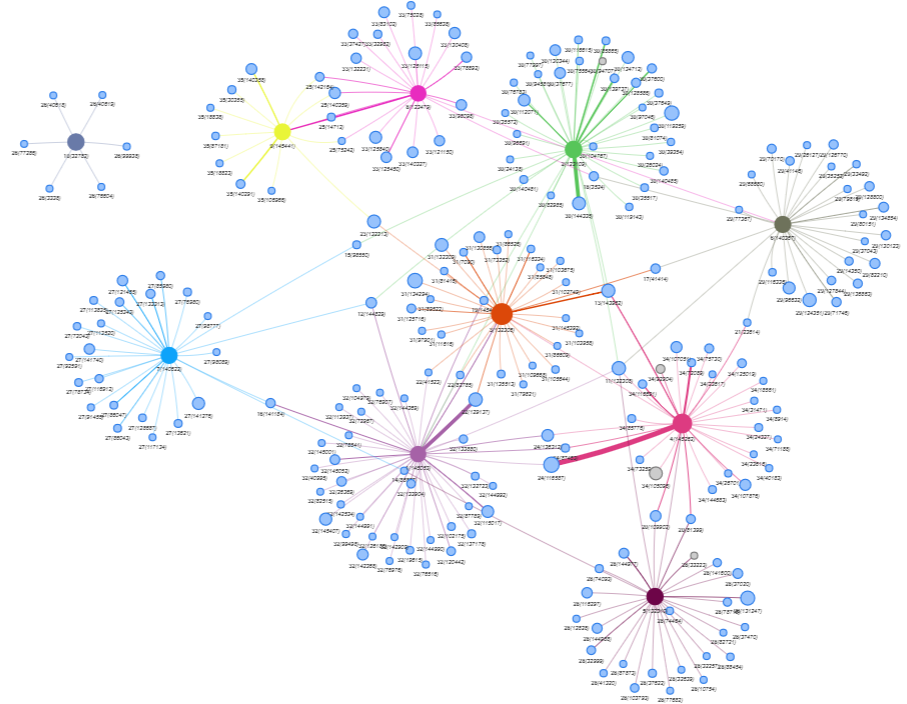
\includegraphics[width=0.75\linewidth]{grafo-10-completo-ConColor.png}
	\caption{10 personas con más casos en Coirón, con sus relaciones. Se agrega detección de comunidades por color.} 
	\label{fig:grafo-10-completo-ConColor}
\end{figure}
